%%
%% Copyright 2007, 2008, 2009 Elsevier Ltd
%%
%% This file is part of the 'Elsarticle Bundle'.
%% ---------------------------------------------
%%
%% It may be distributed under the conditions of the LaTeX Project Public
%% License, either version 1.2 of this license or (at your option) any
%% later version.  The latest version of this license is in
%%    http://www.latex-project.org/lppl.txt
%% and version 1.2 or later is part of all distributions of LaTeX
%% version 1999/12/01 or later.
%%
%% The list of all files belonging to the 'Elsarticle Bundle' is
%% given in the file `manifest.txt'.
%%

%% Template article for Elsevier's document class `elsarticle'
%% with numbered style bibliographic references
%% SP 2008/03/01
%%
%%
%%
%% $Id: elsarticle-template-num.tex 4 2009-10-24 08:22:58Z rishi $
%%
%%
\documentclass[12pt]{elsarticle}

%% Use the option review to obtain double line spacing
%% \documentclass[preprint,review,12pt]{elsarticle}

%% Use the options 1p,twocolumn; 3p; 3p,twocolumn; 5p; or 5p,twocolumn
%% for a journal layout:
%% \documentclass[final,1p,times]{elsarticle}
%% \documentclass[final,1p,times,twocolumn]{elsarticle}
%% \documentclass[final,3p,times]{elsarticle}
%% \documentclass[final,3p,times,twocolumn]{elsarticle}
%% \documentclass[final,5p,times]{elsarticle}
%% \documentclass[final,5p,times,twocolumn]{elsarticle}

%% if you use PostScript figures in your article
%% use the graphics package for simple commands
%% \usepackage{graphics}
%% or use the graphicx package for more complicated commands
\usepackage{graphicx}
\usepackage{float}
%% or use the epsfig package if you prefer to use the old commands
%% \usepackage{epsfig}

%% The amssymb package provides various useful mathematical symbols
%\usepackage{amssymb}
%% The amsthm package provides extended theorem environments
%% \usepackage{amsthm}

%% The lineno packages adds line numbers. Start line numbering with
%% \begin{linenumbers}, end it with \end{linenumbers}. Or switch it on
%% for the whole article with \linenumbers after \end{frontmatter}.
%% \usepackage{lineno}

%% natbib.sty is loaded by default. However, natbib options can be
%% provided with \biboptions{...} command. Following options are
%% valid:

%%   round  -  round parentheses are used (default)
%%   square -  square brackets are used   [option]
%%   curly  -  curly braces are used      {option}
%%   angle  -  angle brackets are used    <option>
%%   semicolon  -  multiple citations separated by semi-colon
%%   colon  - same as semicolon, an earlier confusion
%%   comma  -  separated by comma
%%   numbers-  selects numerical citations
%%   super  -  numerical citations as superscripts
%%   sort   -  sorts multiple citations according to order in ref. list
%%   sort&compress   -  like sort, but also compresses numerical citations
%%   compress - compresses without sorting
%%
%% \biboptions{comma,round}

% \biboptions{}

\journal{Computational and Applied Mathematics}

\begin{document}

\begin{frontmatter}

%% Title, authors and addresses

%% use the tnoteref command within \title for footnotes;
%% use the tnotetext command for the associated footnote;
%% use the fnref command within \author or \address for footnotes;
%% use the fntext command for the associated footnote;
%% use the corref command within \author for corresponding author footnotes;
%% use the cortext command for the associated footnote;
%% use the ead command for the email address,
%% and the form \ead[url] for the home page:
%%

\title{Solving a Suite of NIST Benchmark \\Problems with Hermes}

%% use optional labels to link authors explicitly to addresses:
\author[label1]{Zhonghua Ma}
\ead{mazhonghua83@gmail.com}
\author[label2]{Lukas Korous}
\ead{lukas.korous@gmail.com}
\author[label3]{Erick Santiago}
\ead{laviticus@sbcglobal.net}
\address[label1]{China University of Petroleum, Beijing, China}
\address[label2]{Charles University, Prague, Czech Republic}
\address[label3]{University of Nevada, Reno, USA}

\begin{abstract}
Adaptive grid refinement is a critical component of algorithms for the numerical solution of partial differential equations (PDEs).
The development of new algorithms and computer
codes for the solution of PDEs usually involves the use of proof-of-concept test problems.
It is common to compare different algorithms using a large test set, to evaluate the algorithm's overall quality, which lies in the ability to handle all kinds of problems, and also to determine the algorithm's strengths and weaknesses.
In this paper we solve a set of benchmark problems devised by
W. Mitchell at NIST \cite{mitchell-1}.
The problems exhibit various types of singularities, disruptions, and oscillations.
Each of the benchmark problem is introduced, together with its exact solution.
Then the solution obtained with the use of the multi-platform open source
C++ library for rapid development of adaptive $hp$-FEM and $hp$-DG solvers {\sc Hermes}\footnote{http://hpfem.org/hermes} is shown,
complemented with convergence graphs and comparison of the fully anisotropic
$hp$-FEM to low-order FEM in terms of convergence.
Overview of Hermes is given in the appendix.
\end{abstract}

\begin{keyword}
$hp$-FEM \sep FEM benchmark \sep anisotropic solution \sep test problems \sep finite element method \sep Hermes \sep Hermes2D
%% keywords here, in the form: keyword \sep keyword
%% MSC codes here, in the form: \MSC code \sep code
%% or \MSC[2008] code \sep code (2000 is the default)
\end{keyword}

\end{frontmatter}

%%
%% Start line numbering here if you want
%%
% \linenumbers

%% main text
\section{Introduction}
\label{sec:intro}

The number of adaptive Finite Element codes is growing.
There is no common approach to test adaptive
Finite Element algorithms. The obstacle in developing such an approach is that
the codes differ in application platforms, ways of loading the physical model,
grid formats, boundary conditions handling, input/output formats and the list could go on.

Moreover, some Finite Element codes are specifically designed to be used for
a narrow profile of problems, which also limits the possibility of comparing
their performance on a single problem.
For instance, some of them are widely used in the aerospace industry, others are
mostly used in civil engineering, and some e.g. in electronic and electrical engineering.
Therefore, in order to compare efficiency and robustness of the Finite Element
codes, various test problems are required.

For some classical Finite Element problems, pre-processing
needed for various codes differs greatly.
As a result of the differences between the codes,
the same algorithm may give different results and convergency
behavior for the same problem.

The criterion of performance for adaptive algorithms
is the obtained accuracy as a function of the total number
of DOFs (Degrees Of Freedom) and CPU time. However,
this is quite difficult to establish for CPU time because
differences in hardware and operating systems must be taken into account.

At this point we would like to acknowledge the work of
Dr. William Mitchell (NIST) who collected a suite of
twelve benchmarks for adaptive FEM \cite{mitchell-1}.
The aim of these is to compare different algorithms
using a test set of problems with known exact solutions
that are able to test various aspects of automatic
adaptivity in the appropriate manner.

In this paper, we solve the twelve benchmarks.
The test problems and their exact solutions are
formulated in Sections \ref{sec:bench-1} - \ref{sec:bench-12}.
We also present solutions obtained by {\sc Hermes} library (http://hpfem.org/hermes).
{\sc Hermes} is a multi-platform open source C++
library for rapid development of adaptive $hp$-FEM
and $hp$-DG solvers. Each section also contains a short
description of the benchmark problem, then the numerical
results are presented and discussed. Conclusion and outlooks
are offered at the end of the paper.

%%%%%%%%%%%%%%%%%%%%%%%%%%%%%%%%%%%%%%%%%%%%

\section{Benchmark NIST-1 "Analytic Solution"}
\label{sec:bench-1}

This is the first benchmark problem. Its solution is smooth.
The equation solved is the Poisson's equation.

\begin{equation} \label{poisson}
-\Delta u = f
\end{equation}
in the domain $\Omega = (0, 1)^2$, equipped with Dirichlet
boundary condition given by the exact solution.
The exact solution is $u(x, y) = 2^{4p}x^{p}(1-x)^{p}y^{p}(1-y)^{p}$.
%The right-hand side $f$ is calculated by inserting exact solution into (\ref{poisson}).
The solution of NIST-1 is shown in Fig. \ref{fig:sln-nist01}.
Here $p$ is a parameter, determining the polynomial degree of the exact solution.

\begin{figure}[H]
\centering
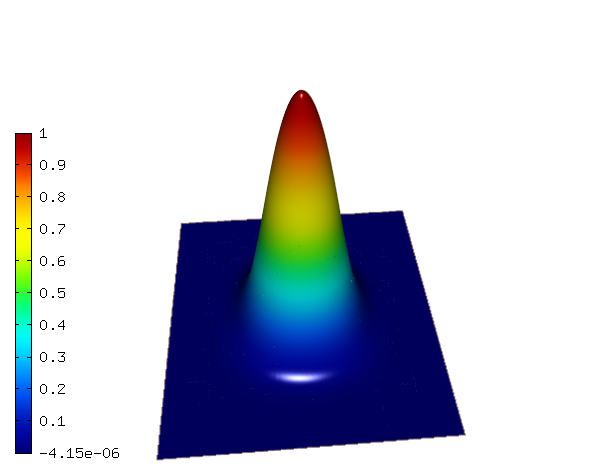
\includegraphics[height=4cm]{nist/nist-1/solution.png}
\caption{The solution to NIST-1 benchmark problem.}
\label{fig:sln-nist01}
\end{figure}

\begin{figure}[H]
\centering
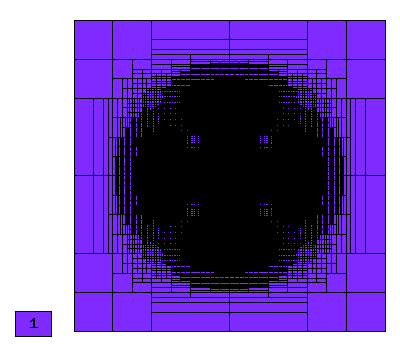
\includegraphics[height=3.7cm]{nist/nist-1/mesh_h1_aniso.png}
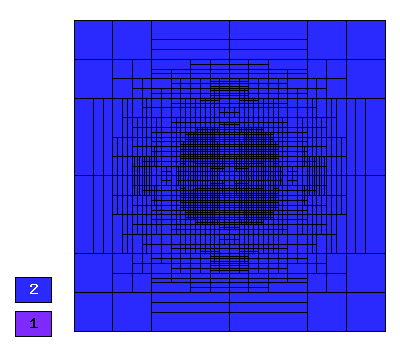
\includegraphics[height=3.7cm]{nist/nist-1/mesh_h2_aniso.png}
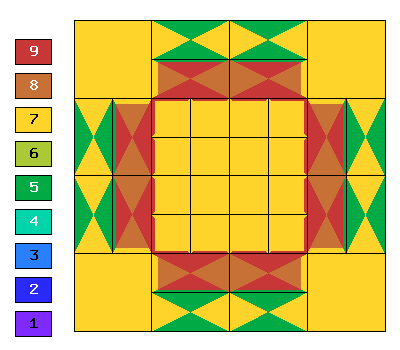
\includegraphics[height=3.7cm]{nist/nist-1/mesh_hp_aniso.png}
\caption{
Final mesh (left) with 51365 DOF and the resulting
relative error estimate in $H^1$-norm of 5.87223e-01 \% for $h$-FEM with linear elements.
Final mesh (middle) with 43401 DOF and the resulting
relative error estimate in $H^1$-norm of 1.37127e-02 \% for $h$-FEM with quadratic elements.
Final mesh (right) with 769 DOF and the resulting
relative error estimate in $H^1$-norm of 4.69543e-03 \% for $hp$-FEM with anisotropic refinements.}
\label{fig:nist-1-hp-aniso}
\end{figure}

Figs. \ref{fig:nist-1-conv} compare all
three approaches to automatic adaptivity from the point
of view of DOF and CPU convergence.

\begin{figure}[H]
\centering
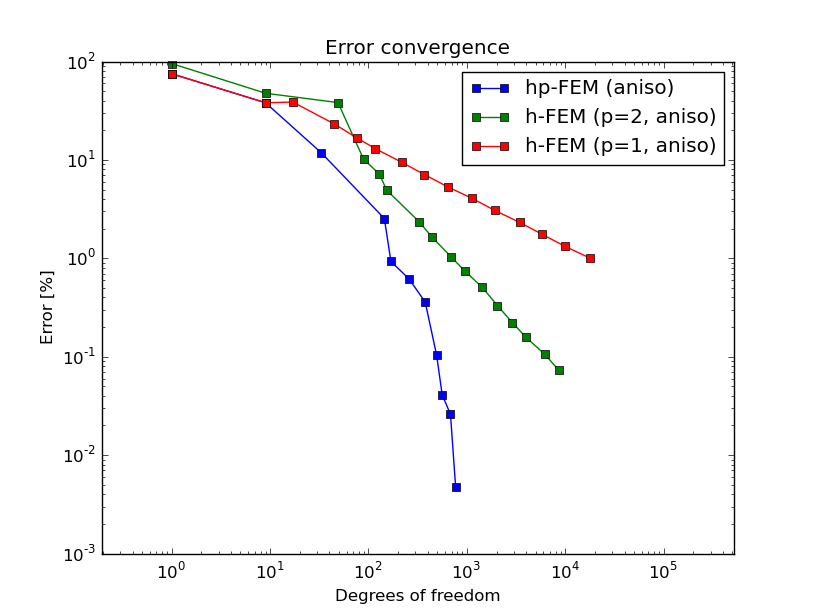
\includegraphics[height=4cm]{nist/nist-1/conv_dof_aniso.png}\ \
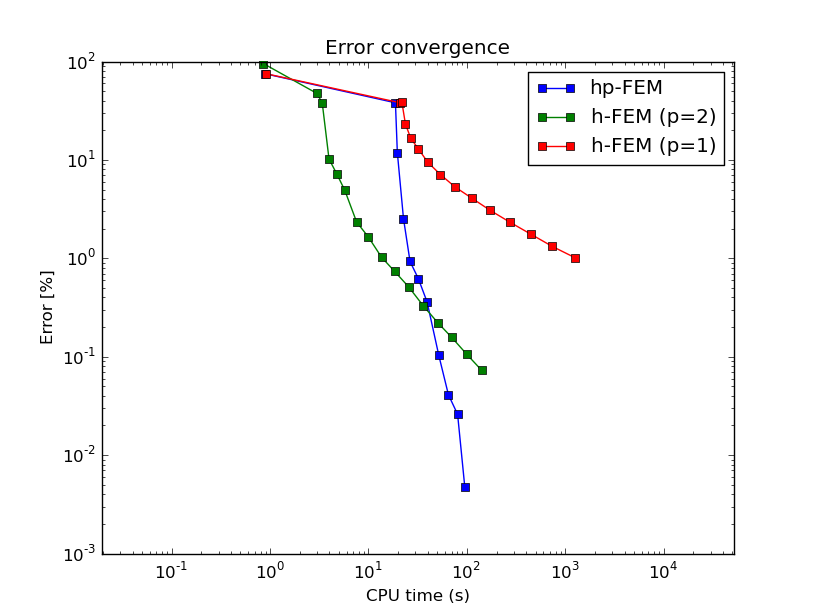
\includegraphics[height=4cm]{nist/nist-1/conv_cpu_aniso.png}
%\vspace{-5mm}
\caption{DOF and CPU time convergence graphs.}
%\vspace{-5mm}
\label{fig:nist-1-conv}
\end{figure}

%%%%%%%%%%%%%%%%%%%%%%%%%%%%%%%%%%%%%%%%%%%%%%%%%%

\section{Benchmark NIST-2 "Reentrant Corner"}
\label{sec:bench-2}

This is a standard benchmark for adaptive FEM algorithms.
The exact solution of this problem is smooth but it contains
singular gradient in the reentrant corner.
The equation solved is the Laplace's equation.

\begin{equation} \label{laplace}
-\Delta u = 0
\end{equation}
in the domain $\Omega = (-1, 1)^2$, with a unit square
section removed from the bottom part of the positive $x$ axis.
Equation (\ref{laplace}) equipped with Dirichlet
boundary conditions given by the exact solution
$u(x, y) = r^{\alpha}\sin(\alpha \theta)$,
where $\alpha = \pi / \omega$, $r = \sqrt{x^2+y^2}$,
and $\theta = tan^{-1}(y/x)$. Here $\omega $ determines
the angle of the reentrant corner.
The solution of NIST-2 with $\omega = 3 \pi / 2$
is shown in Fig. \ref{fig:sln-nist02}.

\begin{figure}[H]
\centering
%\vspace{-5mm}
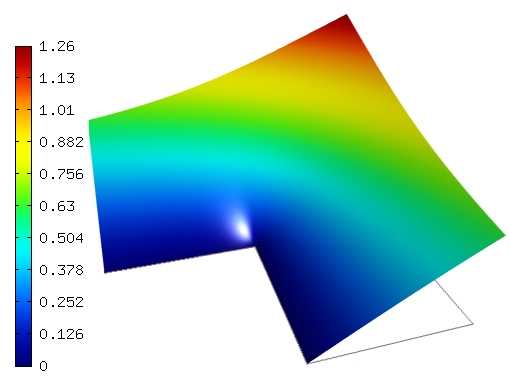
\includegraphics[height=4.5cm]{nist/nist-2/solution.png}
%\vspace{-5mm}
\caption{The solution to NIST-2 benchmark problem.}
%\vspace{-5mm}
\label{fig:sln-nist02}
\end{figure}

\begin{figure}[H]
\centering
%\vspace{-5mm}
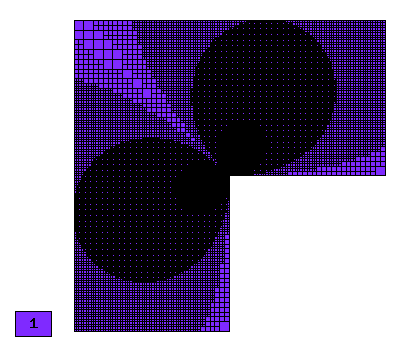
\includegraphics[height=3.7cm]{nist/nist-2/mesh_h1_aniso.png}
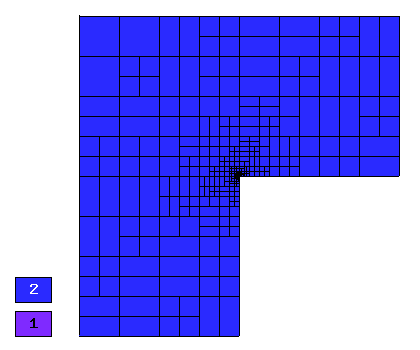
\includegraphics[height=3.7cm]{nist/nist-2/mesh_h2_aniso.png}
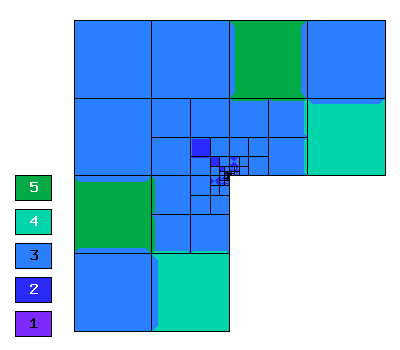
\includegraphics[height=3.7cm]{nist/nist-2/mesh_hp_aniso.png}
%\vspace{-5mm}
\caption{
Final mesh (left) with 46097 DOF and the resulting
relative error estimate in $H^1$-norm of 1.30193e-01 \% for $h$-FEM with linear elements.
Final mesh (middle) with 1289 DOF and the resulting
relative error estimate in $H^1$-norm of 8.26847e-02 \% for $h$-FEM with quadratic elements.
Final mesh (right) with 622 DOF and the resulting
relative error estimate in $H^1$-norm of 8.15289e-02 \% for $hp$-FEM with anisotropic refinements.}
%\vspace{-5mm}
\label{fig:nist-2-hp-aniso}
\end{figure}

Figs. \ref{fig:nist-2-conv} compare all
three approaches to automatic adaptivity from the point
of view of DOF and CPU convergence.

\begin{figure}[H]
\centering
%\vspace{-5mm}
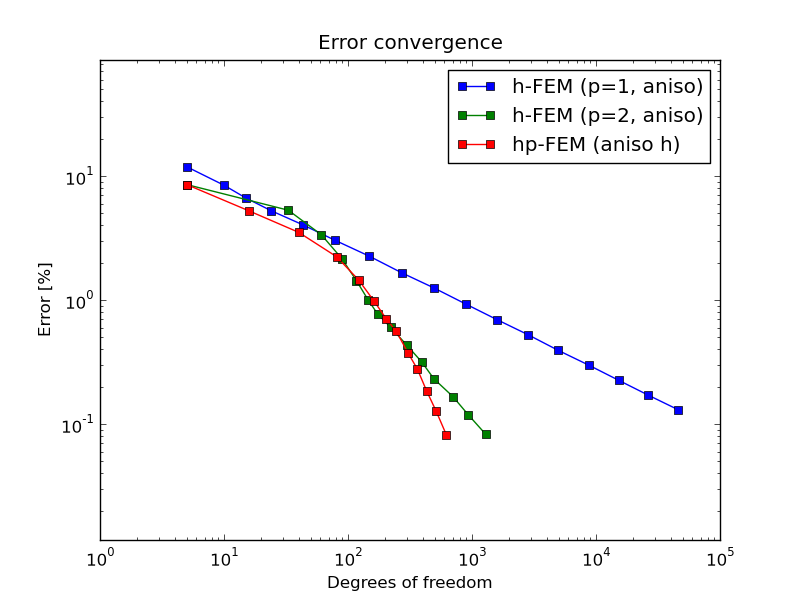
\includegraphics[height=4cm]{nist/nist-2/conv_dof_aniso.png}\ \
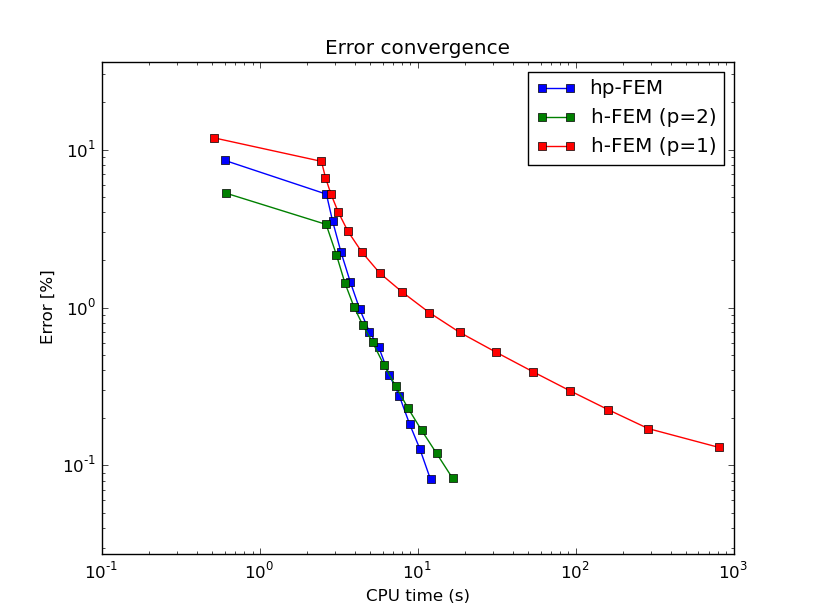
\includegraphics[height=4cm]{nist/nist-2/conv_cpu_aniso.png}
%\vspace{-5mm}
\caption{DOF and CPU time convergence graphs.}
%\vspace{-5mm}
\label{fig:nist-2-conv}
\end{figure}

%%%%%%%%%%%%%%%%%%%%%%%%%%%%%%%%%%%%%%%%%%%%%%%%%%%%%%%

\section{Benchmark NIST-3 "Linear Elasticity"}
\label{sec:bench-3}

Linear elasticity is used extensively in structural analysis
and engineering. Linear elasticity is a simplification
of the general nonlinear equations of elasticity and is the mathematical
study of how solid objects deform and become internally
stressed due to prescribed loading conditions.
In this benchmark, we present a standard system of two
coupled equations with mixed derivative for linear elasticity
in the coupling term. This example employs the adaptive multimesh $hp$-FEM
to solve the equations.

\begin{equation}\label{crack}
\left\{
\begin{array}{l}
\displaystyle
-E \frac{1-\nu^2}{1-2\nu} \frac{\partial^{2} u}{\partial x^{2}} - E\frac{1-\nu^2}{2-2 \nu} \frac{\partial^{2} u}{\partial y^{2}}
-E \frac{1-\nu^2}{(1-2\nu)(2-2\nu)} \frac{\partial^{2} v}{\partial x \partial y} = 0 \\
\displaystyle
-E \frac{1-\nu^2}{2-2\nu} \frac{\partial^{2} v}{\partial x^{2}} - E\frac{1-\nu^2}{1-2\nu} \frac{\partial^{2} v}{\partial y^{2}}
-E \frac{1-\nu^2}{(1-2\nu)(2-2\nu)} \frac{\partial^{2} u}{\partial x \partial y} = 0
\end{array}
\right.
\end{equation}
where $u$ and $v$ are the 
$x$ and $y$ displacements, $E$ is Young's Modulus,
and $\nu$ is Poisson's ratio.

The domain in the example is $\Omega = (-1, 1)^2$ with a slit,
equipped with Dirichlet boundary conditions given by the
exact solution. The exact solution of (\ref{crack}) in polar coordinates is

\[
\left\{
\begin{array}{l}
\displaystyle
u(x, y) = \frac{1}{2G} r^{\lambda}[(k - Q(\lambda + 1))cos(\lambda \theta) - \lambda cos((\lambda - 2) \theta)]  \\
\displaystyle
v(x, y) = \frac{1}{2G} r^{\lambda}[(k + Q(\lambda + 1))sin(\lambda \theta) + \lambda sin((\lambda - 2) \theta)]
\end{array}
\right.
\]
where $\lambda = 0.5444837367825$, $Q = 0.5430755788367$,
$k = 3 - 4 \nu$ and $G = E / (2(1 + \nu))$.
The solution of NIST-3 is shown in Fig. \ref{fig:sln-nist03}.

\begin{figure}[H]
\centering
%\vspace{-5mm}
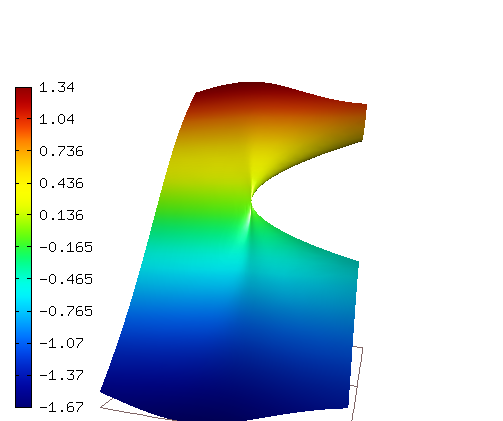
\includegraphics[height=4.5cm]{nist/nist-3/solution-u.png}\ \
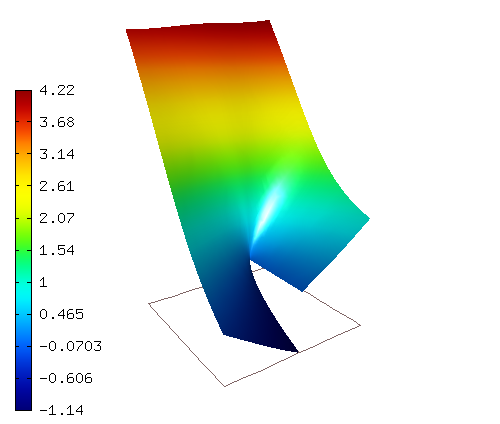
\includegraphics[height=4.5cm]{nist/nist-3/solution-v.png}
%\vspace{-2mm}
\caption{The $u$ (left) and $v$ (right) component to NIST-3 benchmark problem.}
%\vspace{-5mm}
\label{fig:sln-nist03}
\end{figure}

\begin{figure}[H]
\centering
%\vspace{-5mm}
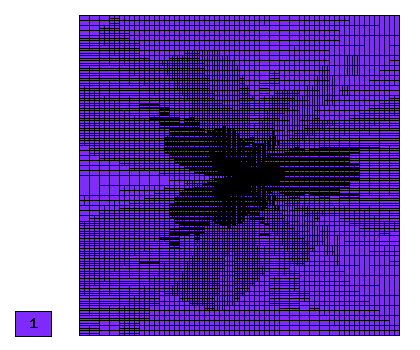
\includegraphics[height=3.7cm]{nist/nist-3/mesh_u_h1_aniso.png}
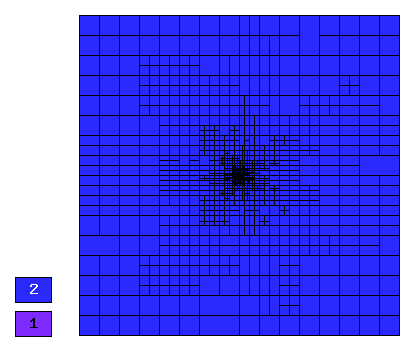
\includegraphics[height=3.7cm]{nist/nist-3/mesh_u_h2_aniso.png}
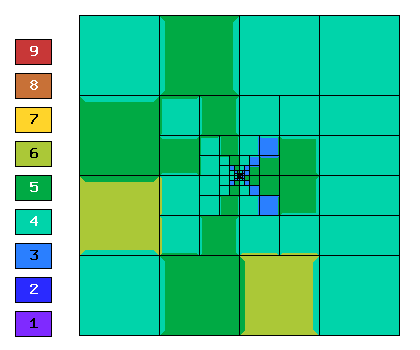
\includegraphics[height=3.7cm]{nist/nist-3/mesh_u_hp_anisoh.png}\ \
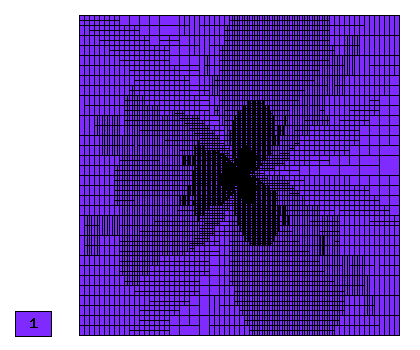
\includegraphics[height=3.7cm]{nist/nist-3/mesh_v_h1_aniso.png}
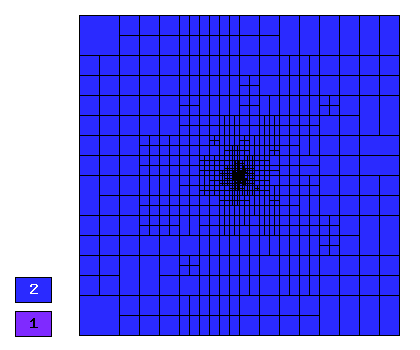
\includegraphics[height=3.7cm]{nist/nist-3/mesh_v_h2_aniso.png}
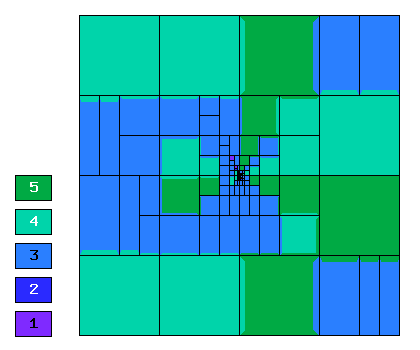
\includegraphics[height=3.7cm]{nist/nist-3/mesh_v_hp_anisoh.png}
%\vspace{-5mm}
\caption{
Final mesh (left) with 39779 DOF and the resulting
relative error estimate in $H^1$-norm of 3.84929e-01 \% for $h$-FEM with linear elements.
Final mesh (middle) with 9330 DOF and the resulting
relative error estimate in $H^1$-norm of 9.56383e-02 \% for $h$-FEM with quadratic elements.
Final mesh (right) with 3897 DOF and the resulting
relative error estimate in $H^1$-norm of 8.05635e-02 \% for $hp$-FEM with anisotropic refinements.}
%\vspace{-5mm}
\label{fig:nist-3-hp-aniso}
\end{figure}

Figs. \ref{fig:nist-3-conv} compare all
three approaches to automatic adaptivity from the point
of view of DOF and CPU convergence.

\begin{figure}[H]
\centering
%\vspace{-5mm}
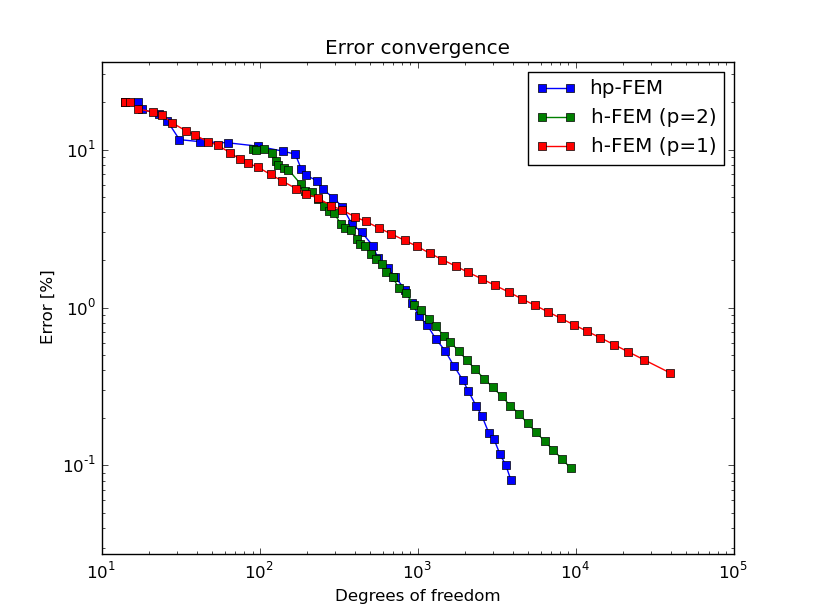
\includegraphics[height=4cm]{nist/nist-3/conv_dof_aniso.png}\ \
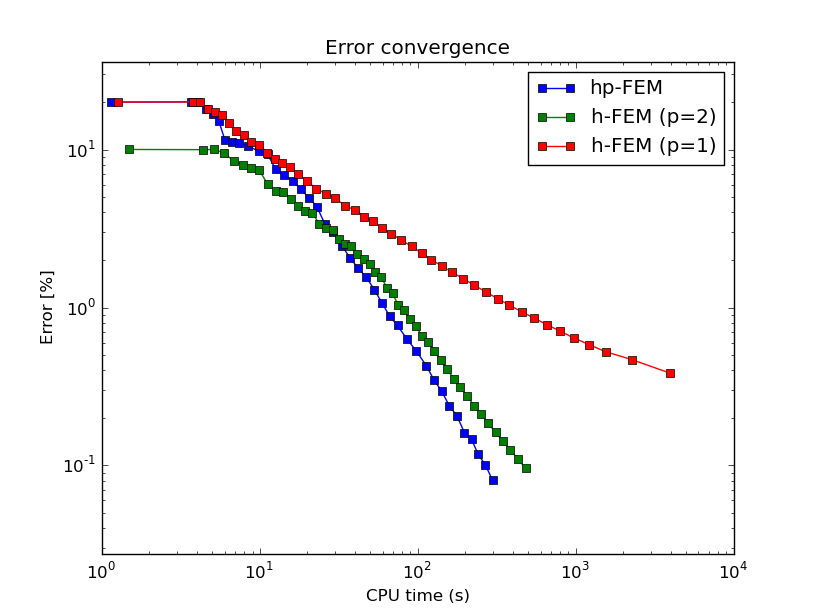
\includegraphics[height=4cm]{nist/nist-3/conv_cpu_aniso.png}
%\vspace{-5mm}
\caption{DOF and CPU time convergence graphs.}
%\vspace{-5mm}
\label{fig:nist-3-conv}
\end{figure}

%%%%%%%%%%%%%%%%%%%%%%%%%%%%%%%%%%%%%%%%%%%%%%%%

\section{Benchmark NIST-4 "Peak"}
\label{sec:bench-4}

The solution of this problem exhibits an exponential peak in the interior of the domain.
The equation solved in this benchmark problem is the Poisson's equation.

\begin{equation} \label{poisson-peak}
-\Delta u = f
\end{equation}
in the domain $\Omega = (0, 1)^2$, equipped with Dirichlet
boundary conditions given by the exact solution.
The exact solution is
$u(x,y) = e^{-\alpha ((x - x_{loc})^{2} + (y - y_{loc})^{2})}$,
where $(x_{loc}, y_{loc})$ is the location of the peak,
and $\alpha$ determines the strength of the peak.
%The right-hand side $f$ is calculated by inserting exact solution into (\ref{poisson-peak}).
The solution of NIST-4 with $\alpha = 1000$,
$(x_{loc}, y_{loc}) = (0.5, 0.5)$ is shown in Fig. \ref{fig:sln-nist04}.

\begin{figure}[H]
\centering
%\vspace{-5mm}
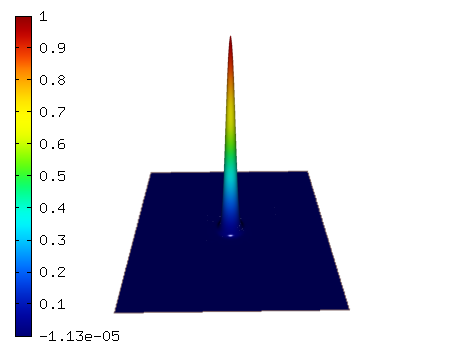
\includegraphics[height=4.5cm]{nist/nist-4/solution.png}
%\vspace{-5mm}
\caption{The solution to NIST-4 benchmark problem.}
%\vspace{-2mm}
\label{fig:sln-nist04}
\end{figure}

\begin{figure}[H]
\centering
%\vspace{-5mm}
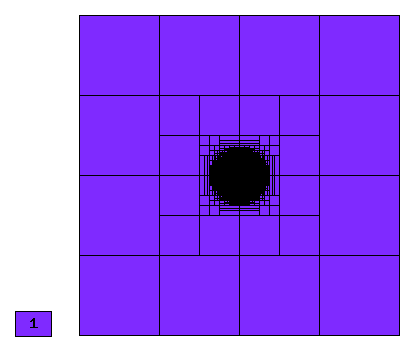
\includegraphics[height=3.7cm]{nist/nist-4/mesh_h1_aniso.png}
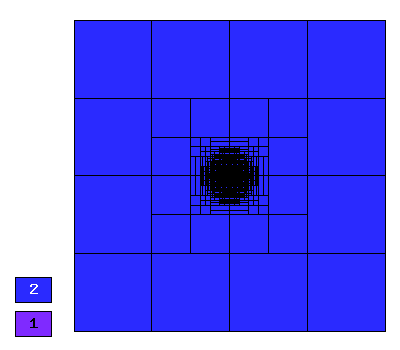
\includegraphics[height=3.7cm]{nist/nist-4/mesh_h2_aniso.png}
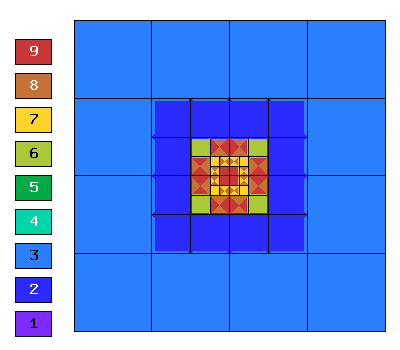
\includegraphics[height=3.7cm]{nist/nist-4/mesh_hp_aniso.png}
%\vspace{-5mm}
\caption{
Final mesh (left) with 58253 DOF and the resulting
relative error estimate in $H^1$-norm of 5.72234e-01 \% for $h$-FEM with linear elements.
Final mesh (middle) with 51473 DOF and the resulting
relative error estimate in $H^1$-norm of 1.39525e-02 \% for $h$-FEM with quadratic elements.
Final mesh (right) with 1561 DOF and the resulting
relative error estimate in $H^1$-norm of 7.02865e-03 \% for $hp$-FEM with anisotropic refinements.}
%\vspace{-5mm}
\label{fig:nist-4-hp-aniso}
\end{figure}

Figs. \ref{fig:nist-4-conv} compare all
three approaches to automatic adaptivity from the point
of view of DOF and CPU convergence.

\begin{figure}[H]
\centering
%\vspace{-5mm}
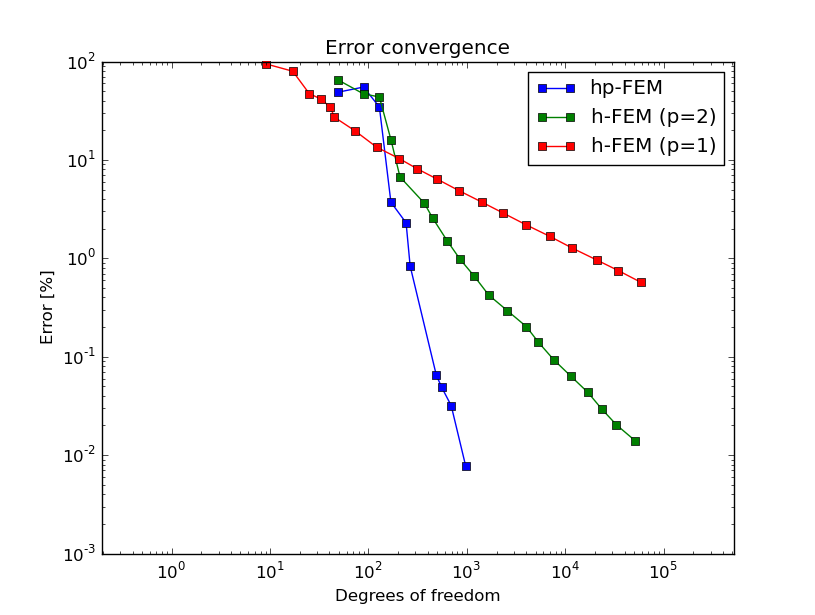
\includegraphics[height=4cm]{nist/nist-4/conv_dof_aniso.png}\ \
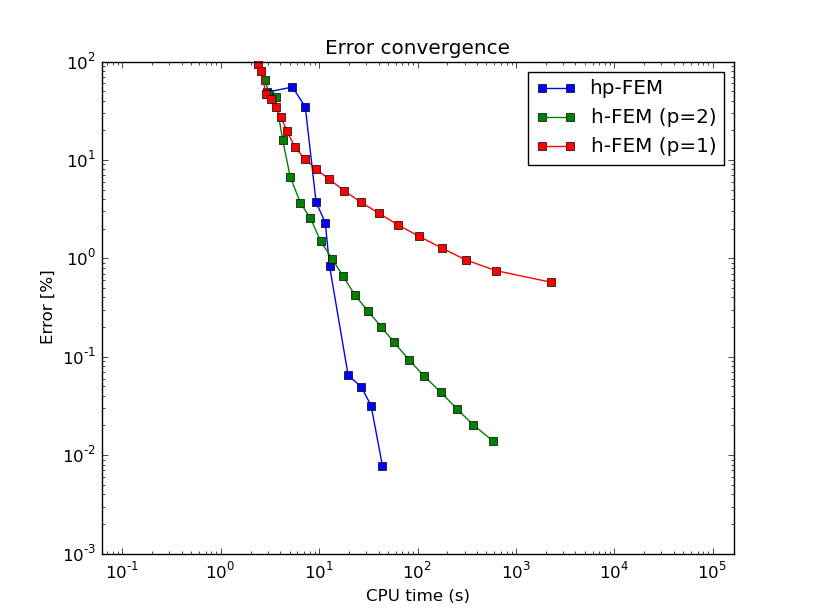
\includegraphics[height=4cm]{nist/nist-4/conv_cpu_aniso.png}
%\vspace{-5mm}
\caption{DOF and CPU time convergence graphs.}
%\vspace{-5mm}
\label{fig:nist-4-conv}
\end{figure}

%%%%%%%%%%%%%%%%%%%%%%%%%%%%%%%%%%%%%%%%%%%%%%%%

\section{Benchmark NIST-5 "Battery"}
\label{sec:bench-5}

This is a heat conduction problem in a nonhomogeneous material.
It comes with an anisotropic solution with strong internal disruption
layers and singularities.
The solution has multiple point singularities in the interior at which
more than three different materials meet. These singularities are stronger than those
corresponding to reentrant corners \cite{demkowicz-1}.
The equation solved is given by

\begin{equation} \label{heat-conduction}
-\frac{\partial }{\partial x}\left(p(x, y)\frac{\partial u}{\partial x}\right)
-\frac{\partial }{\partial y}\left(q(x, y)\frac{\partial u}{\partial y}\right) = f
\end{equation}
in the domain $\Omega = (0, 8.4) \times (0, 24)$. Boundary conditions are zero Neumann on left edge, Newton on the rest of the boundary.
The right-hand side $f$ are constant functions (different in respective materials).
The solution of NIST-5 is shown in Fig. \ref{fig:sln-nist05}.

\begin{figure}[H]
\centering
%\vspace{-5mm}
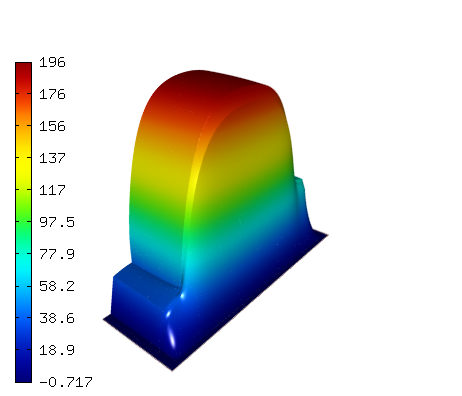
\includegraphics[height=4.5cm]{nist/nist-5/solution.png}
%\vspace{-5mm}
\caption{The solution to NIST-5 benchmark problem.}
\label{fig:sln-nist05}
\end{figure}

\begin{figure}[H]
\centering
%\vspace{-5mm}
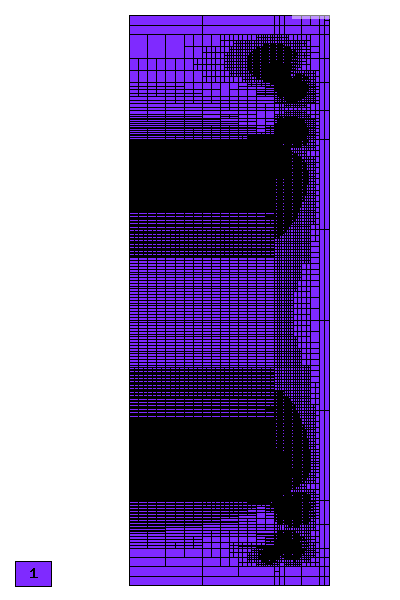
\includegraphics[height=5cm]{nist/nist-5/mesh_h1_aniso.png}
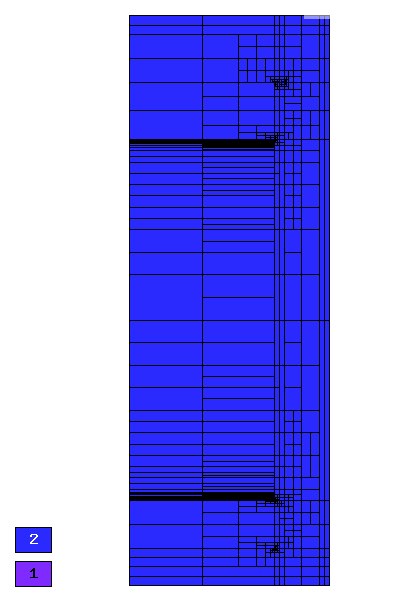
\includegraphics[height=5cm]{nist/nist-5/mesh_h2_aniso.png}
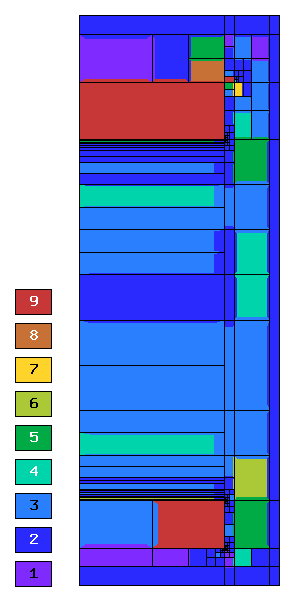
\includegraphics[height=5cm]{nist/nist-5/mesh_hp_aniso.png}
%\vspace{-5mm}
\caption{
Final mesh (left) with 55577 DOF and the resulting
relative error estimate in $H^1$-norm of 9.57345e-02 \% for $h$-FEM with linear elements.
Final mesh (middle) with 12483 DOF and the resulting
relative error estimate in $H^1$-norm of 1.34925e-02 \% for $h$-FEM with quadratic elements.
Final mesh (right) with 7450 DOF and the resulting
relative error estimate in $H^1$-norm of 1.46775e-02 \% for $hp$-FEM with anisotropic refinements.}
%\vspace{-5mm}
\label{fig:nist-5-hp-aniso}
\end{figure}

Figs. \ref{fig:nist-5-conv} compare all
three approaches to automatic adaptivity from the point
of view of DOF and CPU convergence.

\begin{figure}[H]
\centering
%\vspace{-5mm}
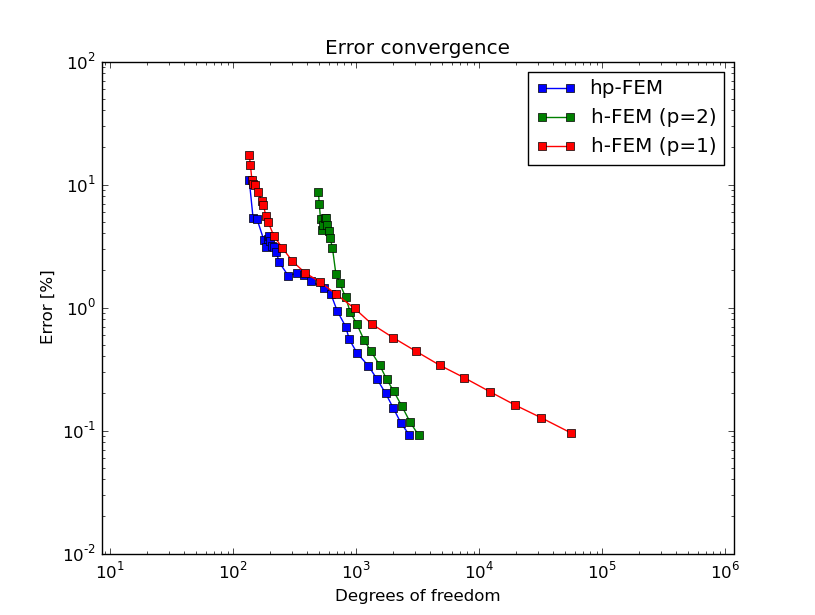
\includegraphics[height=4cm]{nist/nist-5/conv_dof_aniso.png}\ \
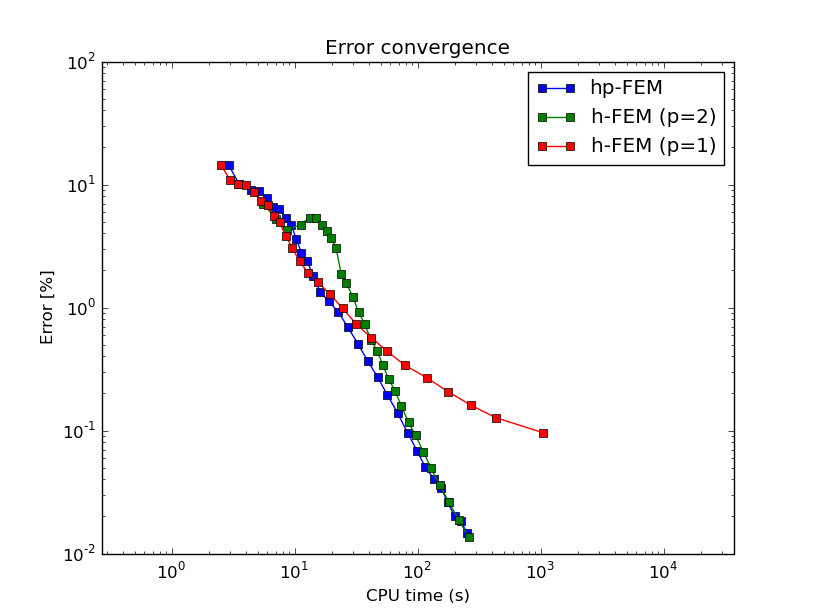
\includegraphics[height=4cm]{nist/nist-5/conv_cpu_aniso.png}
%\vspace{-5mm}
\caption{DOF and CPU time convergence graphs.}
\label{fig:nist-5-conv}
%\vspace{-5mm}
\end{figure}

%%%%%%%%%%%%%%%%%%%%%%%%%%%%%%%%%%%%%%%%%%%%%%%%

\section{Benchmark NIST-6 "Boundary Layer"}
\label{sec:bench-6}

This example is a singularly perturbed problem with known exact solution that exhibits
a boundary layer along the right and top sides of the domain.
It is a convection-diffusion equation with first order terms.

\begin{equation} \label{boundary-layer}
-\epsilon \nabla^{2} u + 2\frac{\partial u}{\partial x} + \frac{\partial u}{\partial y} = f
\end{equation}
in the domain $\Omega = (-1, 1)^2$, equipped with Dirichlet boundary condition
given by the exact solution. The exact solution is
$u(x,y) = (1 - e^{-(1 - x) / \epsilon})(1 - e^{-(1 - y) / \epsilon})cos(\pi (x + y))$,
where $\epsilon$ determines the strength of the boundary layer.
%The right-hand side $f$ is calculated by inserting exact solution into (\ref{boundary-layer}).
The solution of NIST-6 containing a boundary layer
with $\epsilon = 10^{-1}$ is shown in Fig. \ref{fig:sln-nist06}.

\begin{figure}[H]
\centering
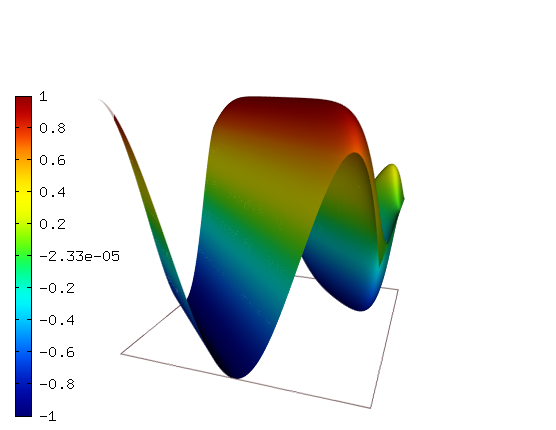
\includegraphics[height=4.5cm]{nist/nist-6/solution.png}
\caption{The solution to NIST-6 benchmark problem.}
\label{fig:sln-nist06}
\end{figure}

\begin{figure}[H]
\centering
%\vspace{-5mm}
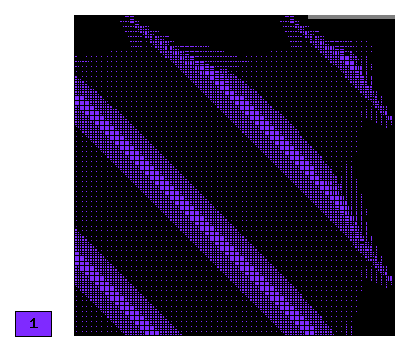
\includegraphics[height=3.7cm]{nist/nist-6/mesh_h1_aniso.png}
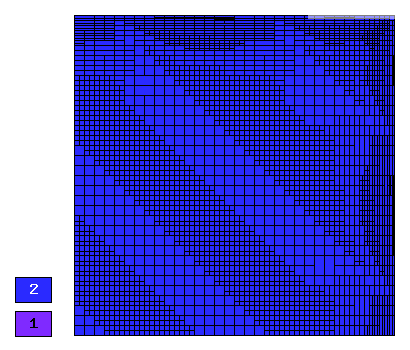
\includegraphics[height=3.7cm]{nist/nist-6/mesh_h2_aniso.png}
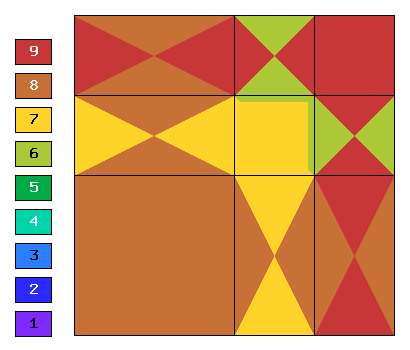
\includegraphics[height=3.7cm]{nist/nist-6/mesh_hp_aniso.png}
%\vspace{-5mm}
\caption{
Final mesh (left) with 55090 DOF and the resulting
relative error estimate in $H^1$-norm of 8.74769e-01 \% for $h$-FEM with linear elements.
Final mesh (middle) with 63145 DOF and the resulting
relative error estimate in $H^1$-norm of 1.46642e-02 \% for $h$-FEM with quadratic elements.
Final mesh (right) with 591 DOF and the resulting
relative error estimate in $H^1$-norm of 6.23458e-04 \% for $hp$-FEM with anisotropic refinements.}
%\vspace{-5mm}
\label{fig:nist-6-hp-aniso}
\end{figure}

Figs. \ref{fig:nist-6-conv} compare all
three approaches to automatic adaptivity from the point
of view of DOF and CPU convergence.

\begin{figure}[H]
\centering
%\vspace{-5mm}
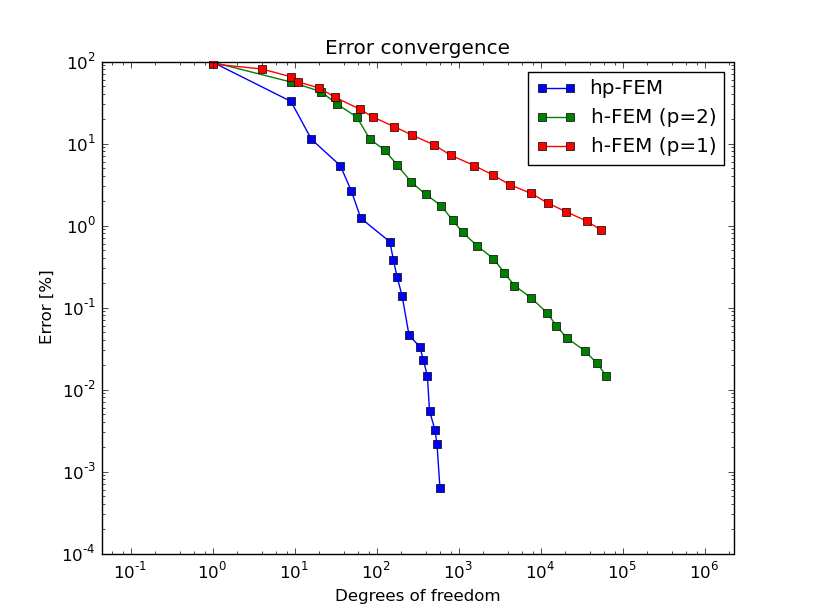
\includegraphics[height=4cm]{nist/nist-6/conv_dof_aniso.png}\ \
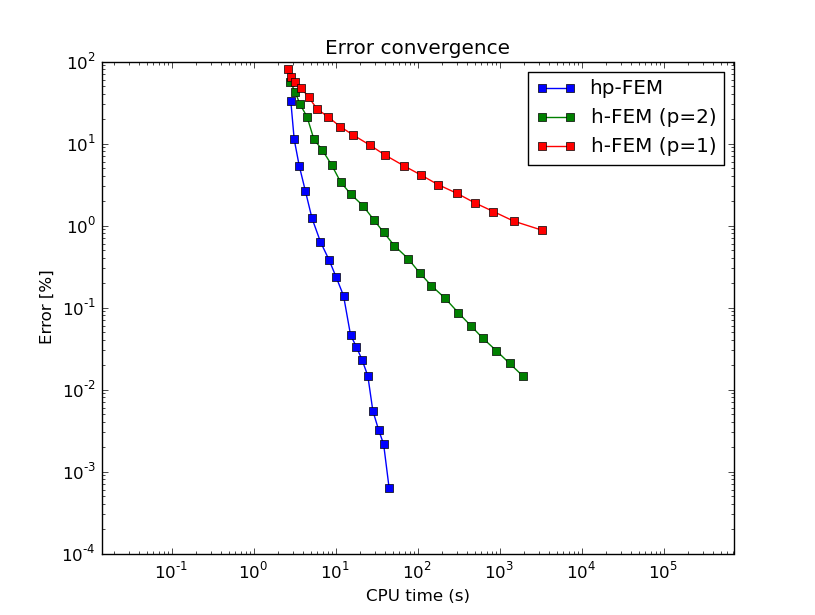
\includegraphics[height=4cm]{nist/nist-6/conv_cpu_aniso.png}
%\vspace{-5mm}
\caption{DOF and CPU time convergence graphs.}
%\vspace{-5mm}
\label{fig:nist-6-conv}
\end{figure}

%%%%%%%%%%%%%%%%%%%%%%%%%%%%%%%%%%%%%%%%%%%%%%%%

\section{Benchmark NIST-7 "Boundary Line Singularity"}
\label{sec:bench-7}

This is a singularity problem with the solution that is singular along the left part of the boundary.
The equation solved in this problem is the Poisson's equation.

\begin{equation} \label{boundary-line-singularity}
-\Delta u = f
\end{equation}
in the domain $\Omega = (0, 1)^2$, equipped with Dirichlet boundary conditions
given by the exact solution. The exact solution is
$u(x,y) = x^{\alpha}$,
where $\alpha \geq 0.5$ determines the strength of the singularity.
%The right-hand side $f$ is calculated by inserting exact solution into (\ref{boundary-line-singularity}).
The solution of NIST-7 with $\alpha = 0.6$ is shown in Fig. \ref{fig:sln-nist07}.

\begin{figure}[H]
\centering
%\vspace{-5mm}
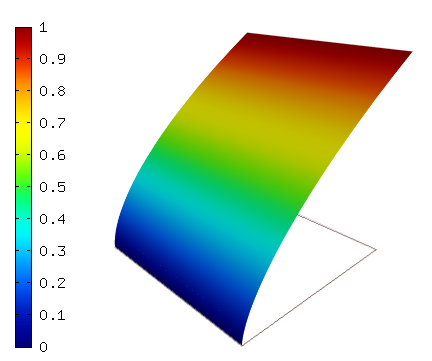
\includegraphics[height=4.5cm]{nist/nist-7/solution.png}
%\vspace{-5mm}
\caption{The solution to NIST-7 benchmark problem.}
%\vspace{-2mm}
\label{fig:sln-nist07}
\end{figure}

\begin{figure}[H]
\centering
%\vspace{-5mm}
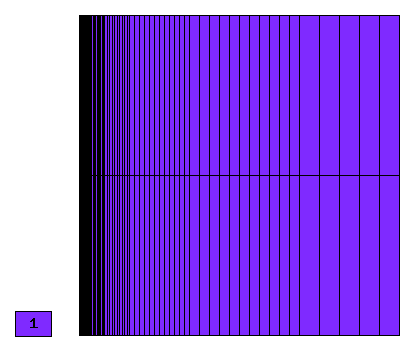
\includegraphics[height=3.7cm]{nist/nist-7/mesh_h1_aniso.png}
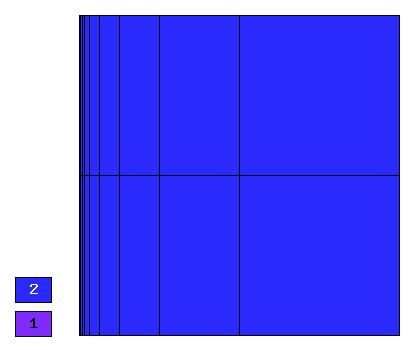
\includegraphics[height=3.7cm]{nist/nist-7/mesh_h2_aniso.png}
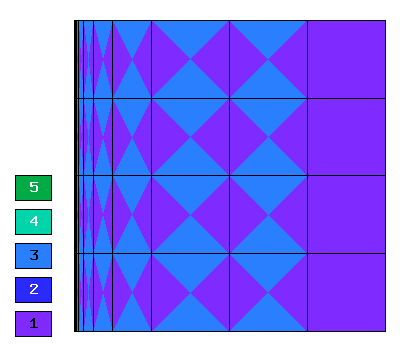
\includegraphics[height=3.7cm]{nist/nist-7/mesh_hp_aniso.png}
%\vspace{-5mm}
\caption{
Final mesh (left) with 684 DOF and the resulting
relative error estimate in $H^1$-norm of 1.45724 \% for $h$-FEM with linear elements.
Final mesh (middle) with 267 DOF and the resulting
relative error estimate in $H^1$-norm of 1.49585 \% for $h$-FEM with quadratic elements.
Final mesh (right) with 88 DOF and the resulting
relative error estimate in $H^1$-norm of 1.46348 \% for $hp$-FEM with anisotropic refinements.}
%\vspace{-5mm}
\label{fig:nist-7-hp-aniso}
\end{figure}

Figs. \ref{fig:nist-7-conv} compare all
three approaches to automatic adaptivity from the point
of view of DOF and CPU convergence.

\begin{figure}[H]
\centering
%\vspace{-5mm}
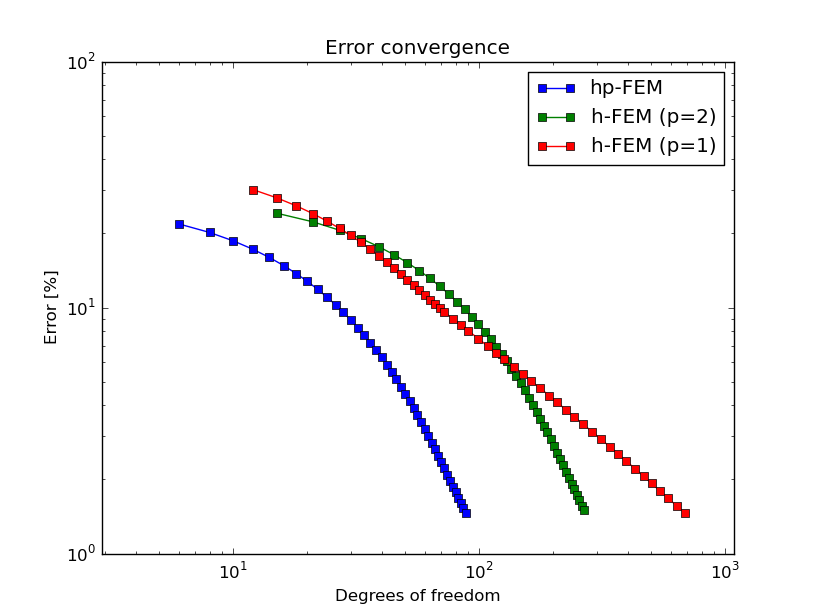
\includegraphics[height=4cm]{nist/nist-7/conv_dof_aniso.png}\ \
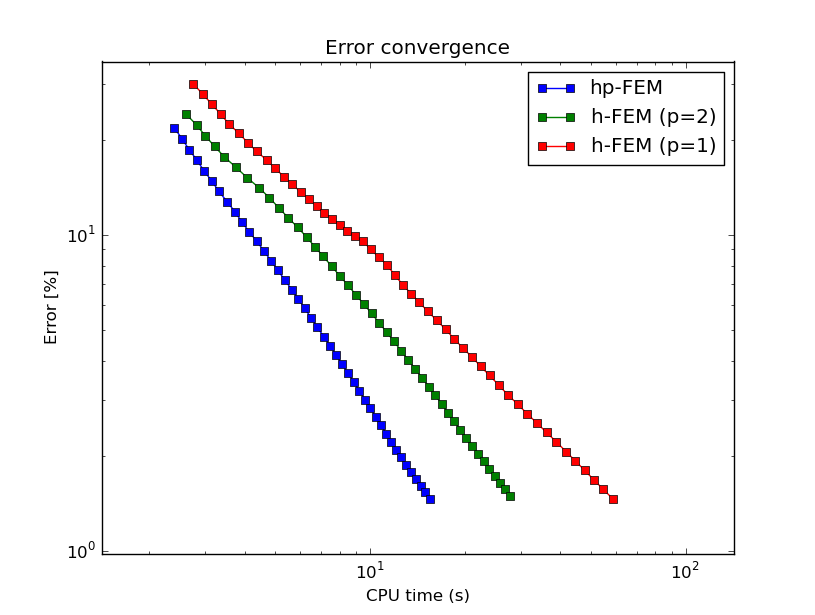
\includegraphics[height=4cm]{nist/nist-7/conv_cpu_aniso.png}
%\vspace{-5mm}
\caption{DOF and CPU time convergence graphs.}
%\vspace{-5mm}
\label{fig:nist-7-conv}
\end{figure}

%%%%%%%%%%%%%%%%%%%%%%%%%%%%%%%%%%%%%%%%%%%%%%%%

\section{Benchmark NIST-8 "Oscillatory"}
\label{sec:bench-8}

This is a wave function that satisfies the Schr\"{o}dinger's equation model of two
interacting atoms, highly oscillatory near the origin.
The equation solved in this problem is the Helmholtz equation.

\begin{equation} \label{oscillatory}
-\nabla^{2} u - \frac{1}{(\alpha + r)^{4}} u = f
\end{equation}
in the domain $\Omega = (0, 1)^2$, equipped with Dirichlet boundary conditions
given by the exact solution. The exact solution is
$u(x,y) = sin(\frac{1}{\alpha + r})$,
where $r = \sqrt{x^{2} + y^{2}}$, $\alpha = 1 / N \pi$ determines the number of oscillations.
%The right-hand side $f$ is calculated by inserting exact solution into (\ref{oscillatory}).
The solution of NIST-8 with $\alpha = 1 / 10 \pi$ is shown in Fig. \ref{fig:sln-nist08}.

\begin{figure}[H]
\centering
%\vspace{-5mm}
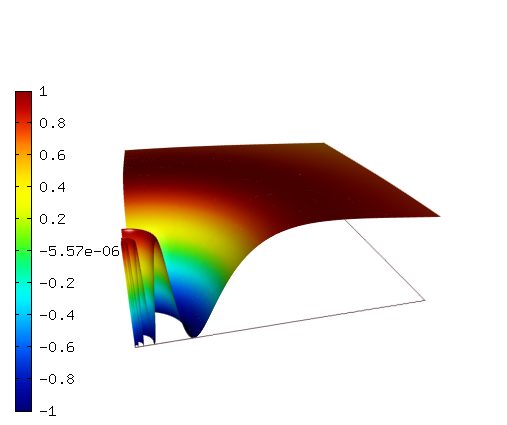
\includegraphics[height=4.5cm]{nist/nist-8/solution.png}
%\vspace{-5mm}
\caption{The solution to NIST-8 benchmark problem.}
%\vspace{-2mm}
\label{fig:sln-nist08}
\end{figure}

\begin{figure}[H]
\centering
%\vspace{-5mm}
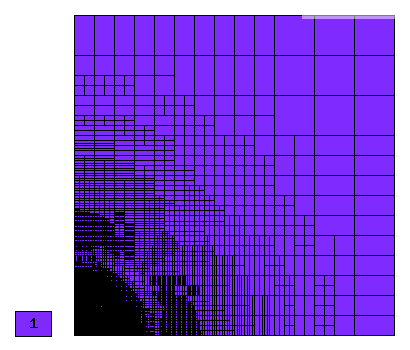
\includegraphics[height=3.7cm]{nist/nist-8/mesh_h1_aniso.png}
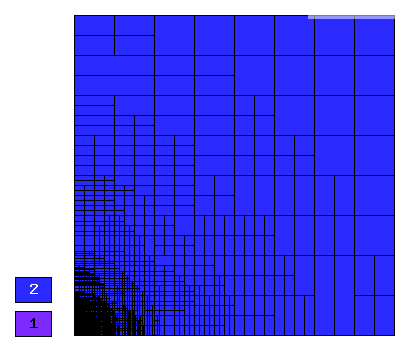
\includegraphics[height=3.7cm]{nist/nist-8/mesh_h2_aniso.png}
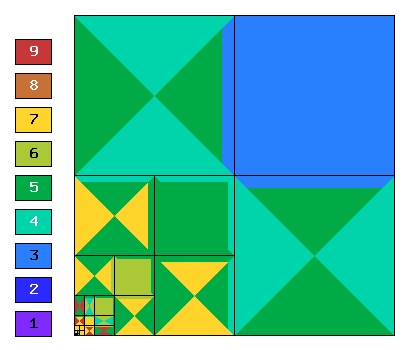
\includegraphics[height=3.7cm]{nist/nist-8/mesh_hp_aniso.png}
%\vspace{-5mm}
\caption{
Final mesh (left) with 55731 DOF and the resulting
relative error estimate in $H^1$-norm of 1.24198 \% for $h$-FEM with linear elements.
Final mesh (middle) with 3413 DOF and the resulting
relative error estimate in $H^1$-norm of 6.64833e-01 1.49585 \% for $h$-FEM with quadratic elements.
Final mesh (right) with 1160 DOF and the resulting
relative error estimate in $H^1$-norm of 9.09848e-02 \% for $hp$-FEM with anisotropic refinements.}
%\vspace{-5mm}
\label{fig:nist-8-hp-aniso}
\end{figure}

Figs. \ref{fig:nist-8-conv} compare all
three approaches to automatic adaptivity from the point
of view of DOF and CPU convergence.

\begin{figure}[H]
\centering
%\vspace{-5mm}
\includegraphics[height=4cm]{nist/nist-8/conv_dof_aniso.png}\ \
\includegraphics[height=4cm]{nist/nist-8/conv_cpu_aniso.png}
%\vspace{-5mm}
\caption{DOF and CPU time convergence graphs.}
%\vspace{-5mm}
\label{fig:nist-8-conv}
%\vspace{-2mm}
\end{figure}

%%%%%%%%%%%%%%%%%%%%%%%%%%%%%%%%%%%%%%%%%%%%%%%%

\section{Benchmark NIST-9 "Wave Front"}
\label{sec:bench-9}

This is a commonly used example for testing the performance of
adaptive refinement algorithms using a wave front and a singularity \cite{mitchell-1, mitchell-2}.
The solution has a sharp circular wave front in the interior of the
domain, with a singularity at the center of the circle.
The equation solved is the Poisson's equation.

\begin{equation} \label{wave-front}
-\Delta u = f
\end{equation}
in the domain $\Omega = (0, 1)^2$, equipped with Dirichlet boundary conditions
given by the exact solution. The exact solution is
$u(x, y) = tan^{-1}(\alpha (r - r_{0}))$,
where $r = \sqrt{(x - x_{loc})^{2} + (y - y_{loc})^{2}}$.
Here $(x_{loc}, y_{loc})$ is the center of the circular wave front,
$r_{0}$ is the distance from the wave front to the center of the circle,
and $\alpha$ gives the steepness of the wave front.
%The right-hand side $f$ is calculated by inserting exact solution into (\ref{wave-front}).
The solution of NIST-9 with $\alpha = 50$, $(x_{loc}, y_{loc}) = (0.5, 0.5)$,
$r_{0} = 0.25$ is shown in Fig. \ref{fig:sln-nist09}.

\begin{figure}[H]
\centering
%\vspace{-5mm}
\includegraphics[height=4.5cm]{nist/nist-9/solution.png}
%\vspace{-5mm}
\caption{The solution to NIST-9 benchmark problem.}
%\vspace{-5mm}
\label{fig:sln-nist09}
\end{figure}

\begin{figure}[H]
\centering
%\vspace{-5mm}
\includegraphics[height=3.7cm]{nist/nist-9/mesh_h1_aniso.png}
\includegraphics[height=3.7cm]{nist/nist-9/mesh_h2_aniso.png}
\includegraphics[height=3.7cm]{nist/nist-9/mesh_hp_aniso.png}
%\vspace{-5mm}
\caption{
Final mesh (left) with 46093 DOF and the resulting
relative error estimate in $H^1$-norm of 1.23973 \% for $h$-FEM with linear elements.
Final mesh (middle) with 4489 DOF and the resulting
relative error estimate in $H^1$-norm of 7.19928e-01 \% for $h$-FEM with quadratic elements.
Final mesh (right) with 1465 DOF and the resulting
relative error estimate in $H^1$-norm of 8.67667e-01 \% for $hp$-FEM with anisotropic refinements.}
%\vspace{-5mm}
\label{fig:nist-9-hp-aniso}
\end{figure}

Figs. \ref{fig:nist-9-conv} compare all
three approaches to automatic adaptivity from the point
of view of DOF and CPU convergence.

\begin{figure}[H]
\centering
%\vspace{-5mm}
\includegraphics[height=4cm]{nist/nist-9/conv_dof_aniso.png}\ \
\includegraphics[height=4cm]{nist/nist-9/conv_cpu_aniso.png}
%\vspace{-5mm}
\caption{DOF and CPU time convergence graphs.}
%\vspace{-5mm}
\label{fig:nist-9-conv}
\end{figure}

%%%%%%%%%%%%%%%%%%%%%%%%%%%%%%%%%%%%%%%%%%%%%%%%

\section{Benchmark NIST-10 "Interior Line Singularity"}
\label{sec:bench-10}

This is another example with anisotropic solution that is suitable for testing
anisotropic element refinements. The equation solved is the Poisson's equation.

\begin{equation} \label{interior}
-\Delta u = f
\end{equation}
in the domain $\Omega = (-1, 1)^2$, equipped with a zero
Neumann boundary condition on left edge, Dirichlet boundary
conditions given by the exact solution on the rest of the boundary.
The exact solution is
$u(x,y) = \cos(Ky)\ (x \le 0)$ and $u(x,y) = \cos(Ky) + x^{\alpha}\ (x > 0)$,
where $K$ and $\alpha$ are constants.
%The right-hand side $f$ is calculated by inserting exact solution into (\ref{interior}).
The solution of NIST-10 containing a line singularity with $K = \pi/2$ and
$\alpha = 2.01$ is shown in Fig. \ref{fig:sln-nist10}.

\begin{figure}[H]
\centering
%\vspace{-5mm}
\includegraphics[height=4cm]{nist/nist-10/solution.png}
%\vspace{-5mm}
\caption{The solution to NIST-10 benchmark problem.}
%\vspace{-5mm}
\label{fig:sln-nist10}
\end{figure}

\begin{figure}[H]
\centering
%\vspace{-5mm}
\includegraphics[height=3.7cm]{nist/nist-10/mesh_h1_aniso.png}
\includegraphics[height=3.7cm]{nist/nist-10/mesh_h2_aniso.png}
\includegraphics[height=3.7cm]{nist/nist-10/mesh_hp_aniso.png}
%\vspace{-5mm}
\caption{
Final mesh (left) with 27999 DOF and the resulting
relative error estimate in $H^1$-norm of 2.87268e-01 \% for $h$-FEM with linear elements.
Final mesh (middle) with 60144 DOF and the resulting
relative error estimate in $H^1$-norm of 2.59816e-04 \% for $h$-FEM with quadratic elements.
Final mesh (right) with 381 DOF and the resulting
relative error estimate in $H^1$-norm of 8.68994e-05 \% for $hp$-FEM with anisotropic refinements.}
%\vspace{-5mm}
\label{fig:nist-10-hp-aniso}
\end{figure}

Figs. \ref{fig:nist-10-conv} compare all
three approaches to automatic adaptivity from the point
of view of DOF and CPU convergence.

\begin{figure}[H]
\centering
%\vspace{-5mm}
\includegraphics[height=4cm]{nist/nist-10/conv_dof_aniso.png}\ \
\includegraphics[height=4cm]{nist/nist-10/conv_cpu_aniso.png}
%\vspace{-5mm}
\caption{DOF and CPU time convergence graphs.}
%\vspace{-5mm}
\label{fig:nist-10-conv}
\end{figure}

%%%%%%%%%%%%%%%%%%%%%%%%%%%%%%%%%%%%%%%%%%%%%%%%

\section{Benchmark NIST-11 "Intersecting Interfaces"}
\label{sec:bench-11}

This is a Poisson's problem with intersecting interfaces,
dividing the plane into four regions.
The solution to this problem contains a severe
singularity that poses a challenge to adaptive methods.
The equation solved is given by

\begin{equation} \label{intersecting}
-\nabla \cdot (a(x,y) \nabla u) = 0
\end{equation}
where the parameter $a$ is piecewise-constant,
$a(x,y) = 161.4476387975881$ in the first and third quadrants,
and $a(x,y) = 1$ in the remaining two quadrants.
The domain of this problem is $\Omega = (-1, 1)^2$, equipped with
Dirichlet boundary conditions given by the exact solution.
The exact solution is
$u(x,y) = r^{a_1} \mu (\theta)$,
where $a_1$ and $\mu (\theta)$ is given in \cite{mitchell-1}.
%The right-hand side $f$ is calculated by inserting exact solution into (\ref{intersecting}).
The solution of NIST-11 is shown in Fig. \ref{fig:sln-nist11}.

\begin{figure}[H]
\centering
%\vspace{-5mm}
\includegraphics[height=4cm]{nist/nist-11/solution.png}
%\vspace{-2mm}
\caption{The solution to NIST-11 benchmark problem.}
%\vspace{-4mm}
\label{fig:sln-nist11}
\end{figure}

\begin{figure}[H]
\centering
%\vspace{-5mm}
\includegraphics[height=3.7cm]{nist/nist-11/mesh_h1_aniso.png}
\includegraphics[height=3.7cm]{nist/nist-11/mesh_h2_aniso.png}
\includegraphics[height=3.7cm]{nist/nist-11/mesh_hp_aniso.png}
%\vspace{-5mm}
\caption{
Final mesh (left) with 46905 DOF and the resulting
relative error estimate in $H^1$-norm of 1.25659 \% for $h$-FEM with linear elements.
Final mesh (middle) with 7777 DOF and the resulting
relative error estimate in $H^1$-norm of 4.73604e-01 \% for $h$-FEM with quadratic elements.
Final mesh (right) with 3459 DOF and the resulting
relative error estimate in $H^1$-norm of 4.7087e-01 \% for $hp$-FEM with anisotropic refinements.}
%\vspace{-5mm}
\label{fig:nist-11-hp-aniso}
\end{figure}

Figs. \ref{fig:nist-11-conv} compare all
three approaches to automatic adaptivity from the point
of view of DOF and CPU convergence.

\begin{figure}[H]
\centering
%\vspace{-5mm}
\includegraphics[height=4cm]{nist/nist-11/conv_dof_aniso.png}\ \
\includegraphics[height=4cm]{nist/nist-11/conv_cpu_aniso.png}
%\vspace{-5mm}
\caption{DOF and CPU time convergence graphs.}
%\vspace{-5mm}
\label{fig:nist-11-conv}
%\vspace{-2mm}
\end{figure}

%%%%%%%%%%%%%%%%%%%%%%%%%%%%%%%%%%%%%%%%%%%%%%%%

\section{Benchmark NIST-12 "Multiple Difficulties"}
\label{sec:bench-12}

This problem combines four aspects of benchmarks
seen in previous sections (nist-2, nist-4, nist-6 and nist-9) into one problem.
The wave front intersects the boundary
layer and corner singularity, and the peak is centered on the wave front.
The equation solved is the Poisson's equation.

\begin{equation} \label{multiple}
-\Delta u = f
\end{equation}
in the L-shaped domain, equipped with Dirichlet boundary conditions
given by the exact solution.
The exact solution is

\[
u(x,y) =  r^{\alpha_{C} }\sin(\alpha_{C} \theta)
+ e^{-\alpha_{P} ((x - x_{P})^{2} + (y - y_{P})^{2})}
+ tan^{-1}(\alpha_{W} (r_{W} - r_{0})) \\
+ e^{-(1 - y) / \epsilon}
\]
where $\alpha_C = \pi / \omega_C$, $r = \sqrt{x^2+y^2}$
and $\theta = tan^{-1}(y/x)$, here $\omega_C$ determines
the angle of the re-entrant corner.
$(x_{P}, y_{P})$ is the location of the peak, $\alpha$
determines the strength of the peak. Furthermore
$r_{W} = \sqrt{(x - x_{W})^{2} + (y - y_{W})^{2}}$,
where $(x_{W}, y_{W})$ is the center of the circular wave front,
$r_{0}$ is the distance from the wave front to the
center of the circle, and $\alpha_W$ gives
the steepness of the wave front. The parameter $\epsilon$ determines the
strength of the boundary layer, the boundary layer was placed on $y = -1$.
%The right-hand side $f$ is calculated by inserting exact solution into (\ref{multiple}).
The solution of NIST-12 with $\omega_C = 3 \pi /2$,
$(x_{W}, y_{W}) = (0, -3/4)$, $r_{0} = 3/4$, $\alpha_{W} = 200$,
$(x_{P}, y_{P}) = (\sqrt{5} / 4, -1/4)$,
$\epsilon = 1/100$ is shown in Fig. \ref{fig:sln-nist12}.

\begin{figure}[H]
\centering
%\vspace{-5mm}
\includegraphics[height=5cm]{nist/nist-12/solution.png}
%\vspace{-5mm}
\caption{The solution to NIST-12 benchmark problem.}
%\vspace{-4mm}
\label{fig:sln-nist12}
\end{figure}

\begin{figure}[H]
\centering
%\vspace{-5mm}
\includegraphics[height=3.7cm]{nist/nist-12/mesh_h1_aniso.png}
\includegraphics[height=3.7cm]{nist/nist-12/mesh_h2_aniso.png}
\includegraphics[height=3.7cm]{nist/nist-12/mesh_hp_aniso.png}
%\vspace{-5mm}
\caption{
Final mesh (left) with 45533 DOF and the resulting
relative error estimate in $H^1$-norm of 2.05698 \% for $h$-FEM with linear elements.
Final mesh (middle) with 10495 DOF and the resulting
relative error estimate in $H^1$-norm of 9.04458e-01 \% for $h$-FEM with quadratic elements.
Final mesh (right) with 4438 DOF and the resulting
relative error estimate in $H^1$-norm of 9.85118e-01 \% for $hp$-FEM with anisotropic refinements.}
%\vspace{-5mm}
\label{fig:nist-12-hp-aniso}
\end{figure}

Figs. \ref{fig:nist-12-conv} compare all
three approaches to automatic adaptivity from the point
of view of DOF and CPU convergence.

\begin{figure}[H]
\centering
%\vspace{-5mm}
\includegraphics[height=4cm]{nist/nist-12/conv_dof_aniso.png}\ \
\includegraphics[height=4cm]{nist/nist-12/conv_cpu_aniso.png}
%\vspace{-5mm}
\caption{DOF and CPU time convergence graphs.}
%\vspace{-5mm}
\label{fig:nist-12-conv}
\end{figure}

%%%%%%%%%%%%%%%%%%%%%%%%%%%%%%%%%%%%%%%%%%%%%%%%%%%%%%%

\section{Conclusion and Outlook}
\label{sec:conclusion}

A challenging set of benchmarks aimed at testing adaptive Finite Element Method implementations in terms of handling diverse problems, and diverse obstacles in their solution, has been presented in this paper.

The solutions and convergence rates obtained by the use of Hermes exemplify that modern adaptive FEM codes can handle a wide range of problems with relative ease.

Hermes also allowed for the comparison of anisotropic hp-FEM to low order (anisotropic) h-FEM. Results of this comparison furnish evidence that hp-FEM consistently outperforms simple h- adaptivity on all kinds of problems, and that hp-FEM can achieve truly exponential convergence.

The numerical results are given in such a way to make it possible to compare them to results obtained with another implementation of adaptive Finite Element Method.

The computations were performed on a standard laptop, with average performance.

\section{Acknowledgment}

This work was supported by Subcontract No. 00089911 of Battelle
Energy Alliance (DOE intermediary) as well as by the
Grant No. IAA100760702 of the Grant Agency of the Academy
of Sciences of the Czech Republic. The first autor was partly
supported by the National Natural Science Foundation
of China under Projects No. 41074099.

\begin{thebibliography}{[KLR73]}

\bibitem{mitchell-1}
W. Mitchell: A Collection of 2D Elliptic Problems for
Testing Adaptive Algorithms, NISTIR 7668, 2010 (available online).

\bibitem{mitchell-2}
W. Mitchell: A Survey of hp-Adaptive Strategies for Elliptic Partial Differential Equations,
Annals of the European Academy of Sciences, to appear (available online).

\bibitem{demkowicz-1}
L. Demkowicz: One and Two Dimensional Elliptic and Maxwell Problems,
Chapman \& Hall \/ CRC Press, Taylor \& Francis, 2006.

%
%\bibitem{label2}
%P. Solin, D. Andrs, J. Cerveny, M. Simko:
%PDE-Independent Adaptive $hp$-FEM Based on Hierarchic Extension of Finite Element Spaces.
%J. Comput. Appl. Math. 233 (2010) 3086-3094.
%
%\bibitem{thermoel}
%P. Solin, J. Cerveny, L. Dubcova, D. Andrs:
%Monolithic Discretization of Linear Thermoelasticity Problems
%via Adaptive Multimesh $hp$-FEM, J. Comput. Appl. Math 234 (2010) 2350 - 2357.
%
%\bibitem{sosedo}
%P. Solin. K. Segeth, I. Dolezel: Higher-Order Finite Element Methods, Chapman \& Hall
%/ CRC Press, Boca Raton, 2003.
\end{thebibliography}

\newpage

\section{Appendix 1 - Automatic hp-adaptivity with the open source library Hermes}

Hermes uses exponentially-convergent adaptive $hp$-FEM and $hp$-DG algorithms where the error drops steadily and fast to the desired accuracy.
Hermes is PDE-independent. Hermes does not employ any technique or algorithm that would limit its applicability to some particular class(es) of PDE problems. Automatic adaptivity is guided by a universal computational a-posteriori error estimate that works in the same way for any PDE.
Hermes has a unique original methodology for handling irregular meshes with arbitrary-level hanging nodes, also various physical fields or solution components in multiphysics problems can be approximated on individual meshes, combining quality $H^1, H(curl), H(div), and L^2$ conforming higher-order elements. The following figure illustrates a coupled problem of heat and moisture transfer in massive concrete walls of a nuclear reactor vessel where all the above features are employed.

For more information about Hermes visit {http://hpfem.org/hermes}.

\begin{figure}[H]
\centering
\includegraphics[height=5cm]{img/hermes_hm_sol.png}
\hspace{10mm}
\includegraphics[height=5cm]{img/hermes_hm_mesh.png}
\caption{Illustration of multimesh hp-FEM.}
\label{fig:hermes_hm}
\end{figure}
\noindent

%% Authors are advised to submit their bibtex database files. They are
%% requested to list a bibtex style file in the manuscript if they do
%% not want to use elsarticle-num.bst.

%% References without bibTeX database:

% \begin{thebibliography}{00}	

%% \bibitem must have the following form:
%%   \bibitem{key}...
%%

% \bibitem{}

% \end{thebibliography}

\end{document}

%%
%% End of file `elsarticle-template-num.tex'.
